%-A Two-Qubit Quantum Processor
%-Building Blocks: Single Qubit Gates, Qubit Readout, Two-Qubit Gate
%-Implementation
%-Frequency Tunability of the Qubits
%  -Decoherence Times
%-Characterization of the Readout
%  -Readout Errors
%-Single Qubit Gates: Tune-Up & Characterization
%-2 Qubit Gate: Tune-Up & Characterization
%-Tests of Entanglement
%  -Entanglement Witnesses
%  -Bell's Inequality
%-2 Qubit Algorithms
%-Grover's Search Algorithm:
%   -Introduction & Background
%   -Implementation
%   -Measurements
%   -Error Analysis
%   -Conclusions

\chapter{Realizing a Two-Qubit Processor}

This chapter discusses the main experimental results of this thesis. We start by discussing the implementation of a superconducting two-qubit processor, discussing the characteristics of the Transmon qubits used in the processor, the readout scheme, single-qubit manipulation, two-qubit gates as well as the experimental procedures used for quantum state and quantum process tomography. The last section of this chapter will discuss the implementation of a quantum algorithm -- so called Grover search algorithm -- using our two-qubit processor and the demonstration of quantum speed-up achieved with our system.

%-Discuss all the experiments performed during the PhD thesis.

\section{Introduction \& Motivation}

\begin{figure}[ht!]
  \centering
	\includegraphics[width=1.\textwidth]{"./material/figures/2-qubit-processor/processor schematic"}
	\caption[Circuit schematic of the two-qubit processor]{The circuit schematic of the two-qubit processor used in this work. Shown are the two Transmon qubits in green, the drive and readout circuit in blue, the fast flux lines in red and the coupling capacitance in magenta.}
	\label{fig:2_qubit_chip_circuit_diagram}
\end{figure}

As discussed in the introduction, the most simple, usable quantum processor contains two qubits that are coupled by an universal two-qubit gate and which in addition can be manipulated and read out individually. We realized such a two-qubit processor using two Transmon qubits, coupled through a fixed capacitance and readout out by individual single-shot readout of the JBA type. The circuit diagram of our processor is shown in fig. \ref{fig:2_qubit_chip_circuit_diagram}, showing the qubits, the drive and readout circuit and the coupling element between them. The following sections we'll discuss the parameters of individual parts of the processor.

\section{Qubit Design}

The parameters of the sample have been chosen in accordance to various design constraints of the qubit processor. For the qubits, the main design goals were high coherence time, good frequency tunability and fast drivability. As we will show later, the coherence time of the qubit is limited by relaxation to the ground state and coupling to external noise sources. The relaxation component of the Transmon qubit is ultimately limited by internal losses of the Josephson junction but usually is bound by coupling to the electromagnetic environment, as will be discussed later. The frequency tunability is important for the realization of fast two-qubit gates but can also limit the relaxation and coherence time of the qubit by coupling to external noise sources. The drivability speed on the other hand is limited by the anharmonicity of the qubit, which can however not be increased arbitrarily since it will make the qubit sensitive to charge noise when chosen too high. For the readout, the main design goals were readout speed and fidelity. The speed of the readout is limited by the quality factor of the readout resonator, which however also can induce qubit relaxation through the Purcell effect and may therefore not be chosen too small.

In the following paragraphs we'll therefore discuss the parameter design for our two-qubit processor and analyze the sample parameters that have been obtained.

\section{Readout Design}

\section{Processor Fabrication}

In this section we will discuss the fabrication of the two-qubit processor realized in this work.

\begin{SCfigure}
	\includegraphics[width=10cm]{"./material/figures/2-qubit-processor/processor photos"}
	\caption{Optical and electron microscope photos of the two-qubit processor realized in this work. a) shows the full processor with the two coupled qubits, fluxlines and readout resonator. b) shows an enlarged version of the central region of the chip with the two qubits and the coupling capacitance. c) Shows a single Transmon qubit.}
	\label{fig:CQED}
\end{SCfigure}

\chapter{Measurement Setup}

\begin{figure}[ht!]
	\centering
		\includegraphics[width=1.\textwidth]{"./material/figures/2-qubit-processor/measurement setup"}
	\caption[The measurement setup used for the two-qubit experiments]{The measurement setup used for the two-qubit experiments. Exactly the same drive and readout scheme is used for both qubits with phase-locked microwave sources and arbitrary waveform generators.}
	\label{fig:MeasurementSetup}
\end{figure}

Fig. \ref{fig:MeasurementSetup} show the measurement setup used for the two-qubit experiments. The different signal and measurement lines as well as the room-temperature and cryogenic microwave components used in our experiments will be described in the following paragraphs.

In this section we discuss the details of the measurement setup used to perform the two-qubit experiments presented in this thesis. All experiments have been performed in a custum-built dilution cryostat at $< 40 \; \mathrm{mK}$ using a cryogenic microwave signal generation and measurement chain. The individual components of this setup will be discussed in the following sections.

\section{Sample Holder \& PCB}

The qubit chip is first glued to a high-frequency PCB \todo{add substrate material details}, then wirebonds are used to connect the groundplane and the center conductors of the on-chip transmission lines to their counterparts on the PCB. Finally, additional bond wires connect isolated ground planes on-chip. The realization of a good and uniform groundplane on the qubit chip and around is very important to supress unwanted resonance modes that can be created when the connection between isolated ground planes is not good enough \todo{Add references e.g. to Schuster's thesis}. The mounted chip on the PCB is then placed in a Copper or Aluminium sample holder which fully encloses the PCB and serves to reduce unwanted couplings to the environment. The coplanar waveguides on the PCB are connected to Mini-SMP cables through a set of connectors that are soldered on the PCB.

\section{Cryogenic Wiring}

For the transmission of microwave signals to our sample we use various types of transmission lines suited for room-temperature and cryogenic application. The main goal of the input lines is to provide adequate signal transmission without introducing too much thermal conductance to the system. For the signal lines that carry the measurement signal from the sample we use superconducting cables \todo{add type} and low-resistance copper cables. In addition, we use superconducting bifilar cables for the DC bias of our magnetic coils. The qubit and fluxline input lines are attenuated and filtered at several stages of the cryostat to reduce signal noise.

\section{Signal Generation \& Acquisition}

Here we discuss the generation and acquisition of the different signals used to manipulate and read out our quantum processor. The experiments that have been performed require the generation, measurement and demodulation of microwave signals, the generation of fast flux control pulses and the application of DC currents to our magnetic coils.

\subsection{Microwave Sideband Mixing}

For qubit manipulation it is often advantageous to use single-sideband mixing for driving the qubit since it can provide higher ON/OFF ratios for microwave pulses and allow the driving of higher qubit-levels using a single, phase-coherent microwave source. To realize this, we use IQ mixers (Hittite \todo{Add exact type number}) that we drive with a continous single-frequency microwave tone and two time-synchronized fast control signals generated by an arbitrary waveform generator (Tektronix AWG5014b). When feeding a signal $LO(t) = i_0 \cos{(\omega_{rf} t )}$ to the LO port of the mixer and two signals $I(t)$, $Q(t)$ to the I and Q ports of the mixer one obtains a signal

\begin{equation}
RF(t) = I(t)\cos{(\omega_{rf} t)}+Q(t)\sin{(\omega_{rf} t)} \label{eq:iqMixer}
\end{equation}

at the LO port of the mixer. Since the IQ mixer that we use is a passive, reciprocal device one can as well feed two input signals to the LO and RF ports and obtain the demodulated signal quadratures at the I and Q ports, a technique that we'll make use of for our qubit readout scheme.

Commercially available IQ mixers often deviate from the ideal behavior as given by eq. (\ref{eq:iqMixer}). Typical imperfections include large insertion losses --i.e. loss of signal power between the different ports of the mixer--, RF signal leakage at zero IQ-input and frequency-dependent phase and amplitude errors of the mixed sideband signals. In order to achieve reliable single-qubit operations we need to correct the signal leakage and quadrature-specific amplitude and phase errors. The signal leakage causes a small part of the LO signal to leak through to the RF port even when the IQ inputs are zeroed. This leakage can be compensated by adding center-frequency $\omega_c$ dependent DC offset voltages to the IQ ports. The appropriate offset voltages can be determined by applying a continuous input signal at a frequency $\omega_c$ to the LO port of the mixer and minimizing the signal power at the RF port by varying the IQ offset voltages. To correct the sideband amplitude and phase errors we apply another correction procedure that we outline here. First, for the signals at the IQ inputs of the mixer we introduce the notation

\begin{equation}
A(t) = I(t)+iQ(t) = a(t)\exp{(-i\phi(t))}
\end{equation}

We consider an IQ signal at a single sideband frequency $\omega_{sb}$ and at fixed complex amplitude $a(t) = a = a_0\exp{(i\phi_0)}$ such that $A(t) = a\exp{(-i \omega_{sb} t)}$. The effect of the gain and phase imperfections of the IQ mixers can then be modeled by assuming that the mixer adds another IQ signal $\epsilon(\omega_{sb},\omega_c)A^*(t)$ at the mirrored sideband frequency $-\omega_{sb}$. We can correct this unwanted signal by adding a small correction $c(\omega_{sb},\omega_c)A^*(t)$ to our IQ input signal. The correction coefficient $c(\omega_{sb},\omega_c)$ usually depends both on the carrier frequency $\omega_c$ and the sideband frequency $\omega_{sb}$. We determine the correction coefficients by generating a continuous waveform at a given center and sideband frequency, measuring the amplitude of the unwanted sideband signal with a fast spectrum analyzer and minimizing its amplitude by varying the correction coefficient $c(\omega_sb,\omega_c)$.

Both the offset and the sideband-amplitude and -phase corrections have been automatized using our data acquisition software, the resulting correction coefficients are summarized in fig. \ref{fig:IQMixerCorrection}.	

\subsection{Fast Magnetic Flux Pulses}

\begin{wrapfigure}{r}{0.6\textwidth}
   \flushright
	 \includegraphics[width=0.6\textwidth]{"./data/ct5/2011_04_04 - flux tomography/flux tomography"}
	 \caption[]{(response function filtered with a Gaussian filter with a cut-off at 0.4 GHz)}
	 \label{fig:FluxLineResponseFunction}
\end{wrapfigure}

The fast flux lines are implemented by a pair of superconducting 50 $\Omega$ transmission lines, which are attenuated by 20 dB and filtered at the 4K and 20 mK stages of the cryostat. The filtering at the 20 mK stage is realized through custom-made, highly absorptive Eccosorb filters. Fig. \ref{fig:EccosorbFilters} shows an image of these filters and the attenuation characteristic obtained. The heavy filtering of the flux line greatly reduces noise seen by the qubit but also distorts all signals sent through the line. This distortion is unwanted especially at high frequencies and needs to be corrected. To do this we need to measure and compensate the frequency response of the flux line at experimental conditions. In order to do this, we feed back the flux signal sent to the sample through a transmission line which is exactly equivalent to the input line. This allows us to measure the returning signal at room temperature and -- assuming symmetric distortion in the input and return line -- to calculate the response function of the input line. Fig. \ref{fig:FluxLineResponseFunction} shows the different parts of the response function of the flux line as measured in our experiment. After eliminating the response of the analog-to-digital converter we can calculate the response function between the input port of the flux line and the sample by solving the equation

\begin{equation}
...
\end{equation}

\subsection{Pulse Synchronization}

\chapter{Measurement Techniques}

In this section we will discuss the techniques used to characterize and manipulate our two-qubit processor. All techniques employed are based on ...

\section{Qubit Readout}

\begin{SCfigure}
\centering
\includegraphics[width=0.5\textwidth]{"./data/ct5/2011_04_21 - grover and tomo/example - qubit 2 s curves"}
\caption[]{Example of a single-qubit s-curve measurement. Shown is the switching probability of the readout for a range of readout drive attenuations, for the different qubit states $\ket{0}$, $\ket{1}$ and $\ket{2}$. The difference in switching probability between individual curves defines the readout contrast between the corresponding qubit states at a given readout power attenuation.}
\label{fig:qubit_scurves_example}
\end{SCfigure}

\section{Qubit Manipulation}

\begin{figure}[ht!]
\centering
\includegraphics[width=1\textwidth]{"./data/ct5/2011_04_21 - grover and tomo/example - qubit 2 spectroscopy"}
\caption[]{Example of a measured qubit spectroscopy. Shown is the switching probability of the qubit readout when driving the qubit with a very long drive pulse (typically 1 $\mu$s) at a given drive frequency. The resonance to the right corresponds to the $\ket{0}\to\ket{1}$ (at frequency $f_{01}$)transition of the qubit, the resonance on the left to the 2-photon $\ket{0}\to\ket{2}$ (at frequency $f_{02}/2$) transition. We perform a Lorentzian fit of the two resonances to obtain the $\ket{0}\to\ket{1}$ and $\ket{0}\to\ket{2}/2$ resonance frequencies, from which we can calculate all other qubit transition frequencies.}
\label{fig:qubit_spectroscopy_example}
\end{figure}

\begin{figure}[ht!]
\centering
\includegraphics[width=1\textwidth]{"./data/ct5/2011_04_21 - grover and tomo/example - qubit 2 rabi"}
\caption[]{Example of a measured qubit Rabi experiment. Shown is the switching probability of the qubit readout when driving the qubit at $f_{01}$ with a Gaussian drive pulse of varying duration. The measurement results are not corrected for readout errors.}
\label{fig:qubit_rabi_example}
\end{figure}


\begin{figure}[ht!]
\centering
\includegraphics[width=1\textwidth]{"./data/ct5/2011_04_21 - grover and tomo/example - qubit 2 ramsey"}
\caption[]{Example of a measured qubit Ramsey experiment. Shown is the switching probability of the qubit readout after performing a $X_{\pi/2}$-wait-$X_{\pi/2}$ drive sequence at a frequency $f_{01}-\delta f$. Fitting the resulting curve with an attenuated sine-wave model allows us to determine the $f_{01}$ frequency of the Qubit with high accuracy.}
\label{fig:qubit_ramsey_example}
\end{figure}

\section{Decoherence Time Measurement}

\chapter{Characterizing the Two-Qubit Processor}

This section discusses the detailed characterization of individual circuit parts that will be used later to realize two-qubit gate and to run a quantum algorithm on the processor. The discussion will focus on the readout and microwave manipulation of the qubits as well as  on the reconstruction of quantum states from measurement data, which will be used later for characterizing gate and processor operation.

\section{Qubit \& Readout Characterization}

\begin{figure}[ht!]
	\centering
		\includegraphics[width=1.\textwidth]{"./data/ct5/2011_04_11 - anticrossing/processor_spectroscopy"}
	\label{fig:ProcessorSpectroscopy}
	\caption[Spectroscopy of the Two-Qubit Processor]{Spectroscopy of the realized two-qubit processor. a) $\ket{0}\to\ket{1}$ and $(\ket{0}\to\ket{2})/2$ transition frequencies of the two qubits with fitted dependence and cavity frequencies. b) Avoided level crossing of the $\ket{01}$ and $\ket{10}$ levels of the qubits with fit, $g = 8.7 \; \mathrm{MHz}$. c) Spectroscopy of qubit 1 at the point indicated in b).}
\end{figure}

The following section discusses the parameters of our two-qubit processor that have been obtained by various measurements.

\subsection{Qubit Parameters}

To obtain all the relevant parameters of our two-qubit processor, we perform a set of measurements from which we obtain the qubit frequencies, anharmonicities, junction asymmetries, the inter-qubit coupling, the coupling to the microwave drive lines, the coupling of each qubit to its readout and the relaxation and dephasing times of the qubits. The drive and readout couplings as well as the relaxation and dephasing times are measured for a range of qubit frequencies, which will allow us later to pick an ideal working point for our two-qubit experiments. The qubit parameters obtained from spectroscopic measurements are as follows:

\begin{itemize}
\item \textit{Qubits}: Spectroscopic measurement of the qubit transitions yielded parameter values of $E_J^I / h = 36.2\; \mathrm{GHz}$, $E_c^I / h = 0.98 \; \mathrm{GHz}$ and $E_J^{II} / h = 43.1\; \mathrm{GHz}$, $E_C^{II} / h = 0.87 \; \mathrm{GHz}$ for the Josephson and charging energies of the two qubits and values of $d^I = 0.2$, $d^{II} =  0.35$ for the qubit junction asymmetries.
\item \textit{Readout resonator}: The frequencies of the readout resonators have been measured as $\nu_R^I = 6.84 \; \mathrm{GHz}$ and $\nu_R^{II} = 6.70 \; \mathrm{GHz}$ with quality factors $Q^I \simeq Q^{II} = 730$, independent measurements of the Kerr nonlinearities yielded $K^I / \nu_R^I \simeq K^{II} / \nu_R^{II} = -2.3\pm 0.5 \times 10^{-5}$ \todo{add junction parameters inferred from the bare resonator frequencies}.
\item \textit{Qubit-Resonator coupling}: The coupling of the qubits to the readout resonators has been spectroscopically determined as $g_0^I \simeq g_0^{II} = 50 \; \mathrm{MHz}$
\end{itemize}

\subsubsection{Readout Parameters}

\subsubsection{Qubit Readout, Driving, Relaxation and Dephasing Time}

\begin{figure}[ht!]
   \centering
	 \includegraphics[width=1\textwidth]{"./data/ct5/qubits - parameter surveys/qubit parameters"}
	 \caption[A qubit parameter survey showing $T_1$, readout contrast and Rabi frequency of the two qubits over a large range of qubit frequencies]{A qubit parameter survey showing the relaxation time $T_1$, the readout contrast and the Rabi frequency at a fixed drive amplitude for the two qubits over a large range of qubit frequencies.}
	 \label{fig:qubit_parameters}
\end{figure}

In order to obtain the relaxation time and the coupling of the qubit to the drive line, we perform an automated survey of qubit spectroscopies, qubit readout characterizations and $T_1$ measurements at different qubit frequencies. The results of such a parameter survey are summarized in fig \ref{fig:qubit_parameters}, showing the relaxation time $T_1$,  the readout contrast $c_{10}$ and the Rabi frequency $f_{Rabi}$ for a fixed drive amplitude for the two qubits in a frequency range between 5.2 and 6.5 GHz. As can be seen, the relaxation time of the qubits tends to increase the farther detuned each qubit is from its readout resonator. Not surprisingly, the drive frequency of the qubit also decreases when the qubit-resonator detuning increases as expected from the Purcell effect, which filters incoming microwave signals that are far-detuned from the resonator frequency. The inverse is true for the readout contrast, which increases near-linearly when reducing the qubit-resonator detuning due to the increase of the dispersive resonator frequency shift induced by the qubit that gets stronger the less the qubit is detuned from the readout resonator.

\smallskip

It is interesting to note the non-monotnous characteristic of the qubit relaxation time $T_1$ shown in fig. \ref{fig:qubit_parameters}, which cannot be explained by Purcell-filtering through the readout resonator and hints at a different qubit relaxation process present in the system. A possible explanation would be the coupling of the qubit to a spurious low-Q resonance in the environment. Coupling to volumetric resonance modes of the sample holder or non-CPW resonance modes of the readout resonator can be possible explanations for the data. Also, the overall dependency of the relaxation time $T_1$ on the qubit-resonator detuning --ignoring the ``fine-structure'' present in the system-- is not quadratic as would be expected from the Purcell theory but rather linear. Also, by comparing the qubit relaxation time to the Rabi drive frequency reveals that the increase in $T_1$ is cleary not proportional to the Purcell factor that determines the qubit relaxation rate through the readout resonator. However, the observed $T_1$ dependency can be partially explained by taking into account the qubit relaxation through the fast fluxline, which might be to strongly-coupled to the qubit on our chip, hence inducing additional qubit relaxation beyond the Purcell and intrinsic qubit relaxation rates. This effect will therefore be studied in more detail in the following sections.

\section{Single-Qubit Operations}

\begin{figure}[ht!]
	\centering
		\includegraphics[width=1.\textwidth]{"./data/ct5/2010_12_01 - iq tomography/iq_tomographies"}
	\caption[Demonstration of single-qubit IQ control]{Demonstration of single-qubit IQ control. The figures show the state probability of a single qubit when preparing it in one of the states $\ket{1}$, $1/\sqrt{2}(\ket{0}+\ket{1})$ or $1/\sqrt{2}(\ket{0}+i\ket{1})$ and subjecting the qubit to a microwave drive pulse of the form $a(t) = V_I\cdot\cos{\omega_{rf}t}+V_Q\cdot\sin{\omega_{rf}t}$.}
	\label{fig:single_qubit_iq_control}
\end{figure}

To perform arbitrary single-qubit operations -- as needed e.g. for implementing a quantum algorithm or performing quantum state tomography -- we need to implement a universal set of $X$, $Y$ and $Z$ qubit gates with our processor. Qubit rotations in the $XY$-plane are implemented through microwave drive pulses, where the phase of the drive pulse in reference to an arbitrary reference determines the rotation axis and the amplitude of the drive pulse the Rabi frequency of the gate. To characterize the drive pulses, we perform an experiment where we initialize a single-qubit in the states $\ket{1}$, $1/\sqrt{2}(\ket{0}+\ket{1})$ and $\sqrt{2}(\ket{0}+i\ket{1})$ and subject it afterwards to a single microwave pulse of the form $a(t) = V_I\cdot\cos{\omega_{rf}t}+V_Q\cdot\sin{\omega_{rf}t}$, which we tune by changing the input voltages $V_I$ and $V_Q$ to the $IQ$-mixer that generates the pulse from a continuous input micrwave-tone at frequency $\omega_{rf}$. We measure the qubit state at different values of $V_I$, $V_Q$, obtaining the graph shown in fig. \ref{fig:single_qubit_iq_control}. The qubit which was prepared in state $\ket{1}$ shows a perfectly cylinder-symmetric switching probability pattern when subjecting it to an IQ-pulse of a given phase, which is what one would expect for a qubit being prepared in either the $\ket{0}$ or $\ket{1}$ state. On the contrary, the switching probability distributions of the measured qubits prepared in the states $1/\sqrt{2}(\ket{0}+\ket{1})$ and $1/\sqrt{2}(\ket{0}+i\ket{1})$ are mirror-symmetric, where the switching probability does not vary at all along the drive axis which corresponds to the axis along which the qubit has been prepared. These measurements demonstrate therefore our ability to prepare and drive the qubit along arbitrary axes of the Bloch sphere. In the following sections we will analyze more in detail the drive errors inherent to our system and quantitatively analyze differnt error sources. 

\subsection{Estimation of drive errors}

Since the Transmon is a weakly anharmonic multi-level system and thus no real qubit, driving the $\ket{0}\to\ket{1}$ transition with high power can induce transitions to higher Transmon levels. It is important to estimate and reduce these errors when performing fast qubit gates e.g. for state preparation or tomography. To model the driving of a Transmon, we use the simple drive model in the rotating-frame approximation and as used e.g. in \cite{motzoi_simple_2009}:

\begin{equation}
\hat{H} = \left(
						 \begin{array}{ccc}
						0 & \epsilon^*(t) & 0 \\
						\epsilon(t) & \delta & \sqrt{2}\epsilon^*(t) \\
						0 & \sqrt{2}\epsilon(t) & 2\delta + \alpha
						\end{array}
					\right)
\end{equation}

Here, $\epsilon(t) = \epsilon_x(t)+i\epsilon_y(t)$ is the complex drive IQ amplitude in the rotating qubit frame, $\delta$ is the detuning of the microwave drive from the Transmon $\omega_{01}$ transition frequency and $\alpha$ is the Tranmon anharmonicity. To estimate the leakage

\section{Two Qubit Operations}

\subsection{Creation of Entanglement}

\begin{figure}
	\centering
		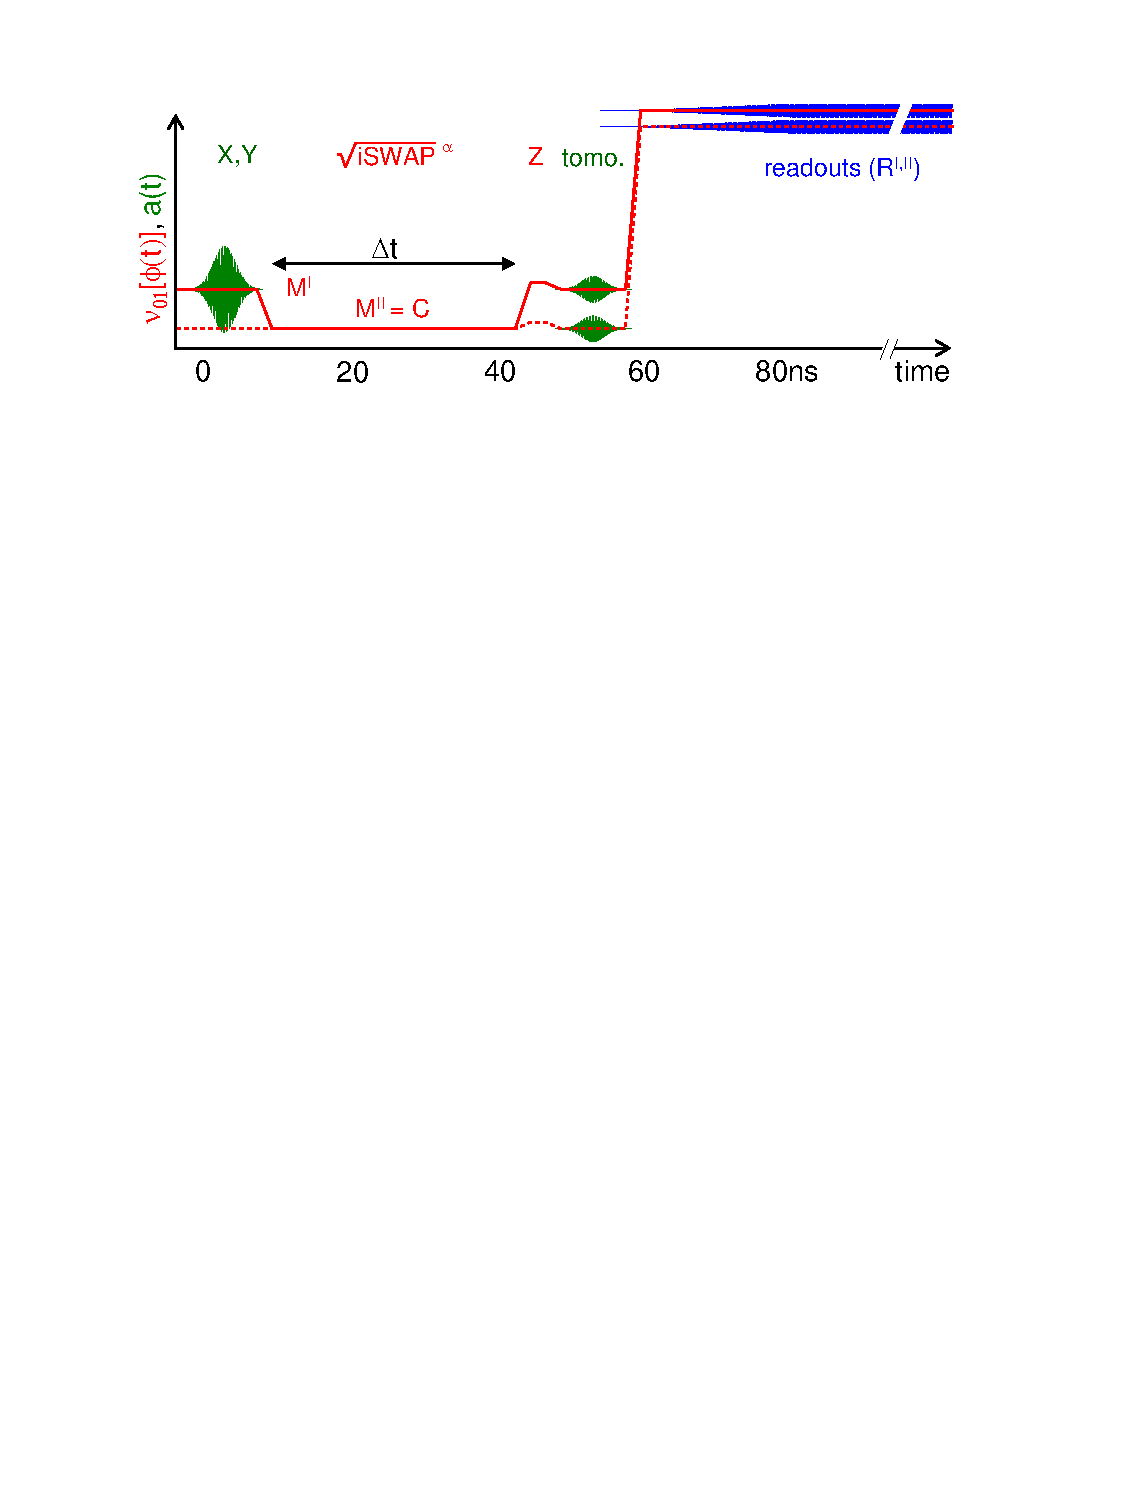
\includegraphics[width=0.8\textwidth]{./material/papers/iswap/figures/iswap_gate_pulse_sequence}
	\label{fig:ISwapPulseSequence}
	\caption{}
\end{figure}

\begin{figure}
  \flushright
	\includegraphics[width=1\textwidth]{"./data/ct5/2011_02_09 preparation of bell states/bell matrices"}
	\caption{Experimentially created $\ket{\psi_+}$ ($F = 0.91$) and $\ket{\psi_-}$ ($F=0.93$) states}
	\label{fig:BellStates}
\end{figure}

\subsection{Violation of the Bell Inequality}

\begin{figure}
	\centering
		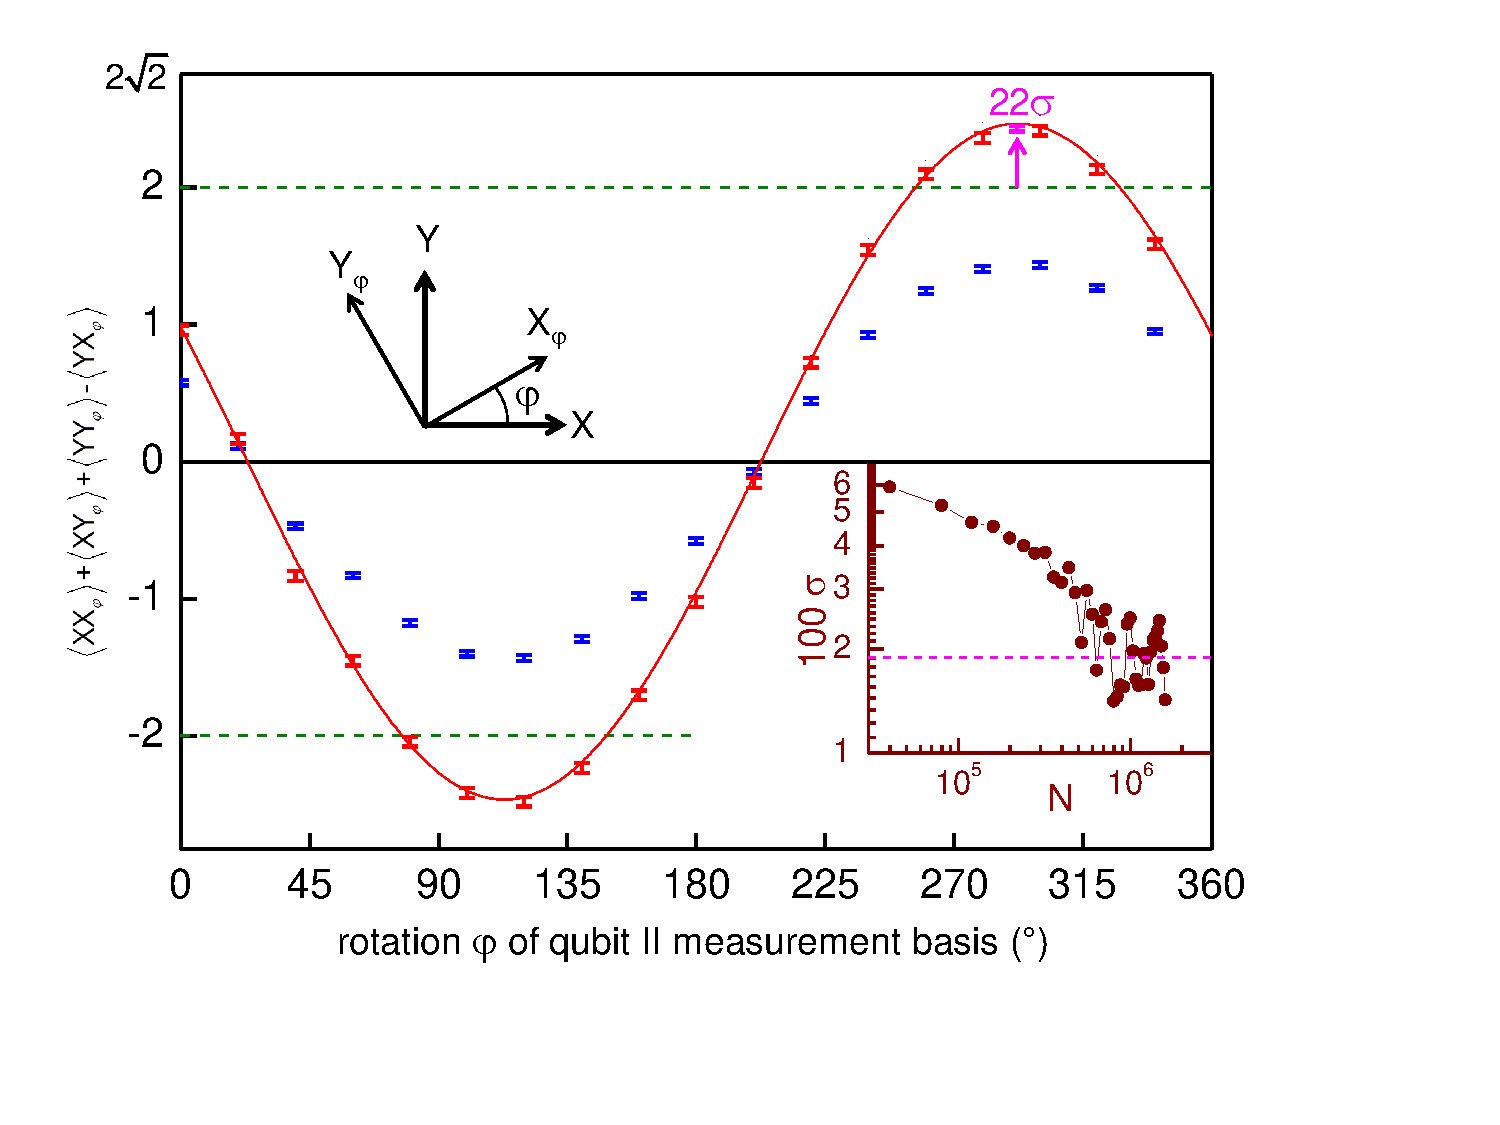
\includegraphics[width=0.8\textwidth]{./material/papers/iswap/figures/chsh}
	\label{fig:CHSH}
	\caption{}
\end{figure}

\begin{equation}
\mathrm{CHSH} = \mathrm{QS}+\mathrm{RS}+\mathrm{RT}-\mathrm{QT}
\end{equation}
with the operators $\mathrm{Q,R,S,T}$ being defined as

\begin{eqnarray}
	\begin{array}{cccccccc}
		\mathrm{Q} & = & \sigma_z^1 &&& \mathrm{S} & = & \sigma_z^2\cdot \cos{\phi}+\sigma_x^2 \cdot \sin{\phi} \\
		\mathrm{R} & = & \sigma_x^1 &&& \mathrm{T} & = & -\sigma_z^2\cdot \sin{\phi}+\sigma_x^2 \cdot \cos{\phi}
	\end{array}
\end{eqnarray} 

Here, the angle $\phi$ is a parameter that should be chosen in accordance to the phase of the Bell state on which it is applied.

\subsection{Quantum State Tomography of Two-Qubit States}

Quantum state tomography is the procedure of experimentally determining an unknown quantum state\citep{michael_a._nielsen_quantum_2000}.

The density matrix of an n-qubit system can be written in general form as
\begin{eqnarray}
\rho & = & \sum\limits_{v_1,v_2\hdots v_n} \frac{c_{v_1,v_2\hdots v_n} \sigma_{v_1}\otimes \sigma_{v_2}\hdots \sigma_{v_n}}{2^n} \label{eq:state_tomography_state_representation} \\
c_{v_1,v_2\hdots v_n} & = & \mathrm{tr}\left(\sigma_{v_1}\otimes \sigma_{v_2}\hdots \otimes\sigma_{v_n} \; \rho \right)  \label{eq:state_tomography_coefficients}
\end{eqnarray}
where $v_i \in \left\{ X,Y,Z,I\right\}$ and $n$ gives the number of qubits in the system and where the $c_{v_1,v_2\hdots v_n}$ are real-valued coefficients that fully describe the given density matrix. To reconstruct the density matrix of an experimental quantum system in a well-prepared state it is therefore sufficient to measure the expectation values of these $n^2-1$ coefficients on an ensemble of identically prepared systems. However, statistical and systematic measurement errors can yield a set of coefficients that corresponds to a {\it non-physical} density matrix which violates either the positivity or unity-trace requirement. In the following paragraph we will therefore discuss a technique with which one can estimate the density matrix of a system in a more correct way.

\subsubsection{Maximum Likelihood Estimation of Quantum States}

A method which is often used in quantum state tomography is the so-called {\it maximum-likelihood} technique. Rather than directly calculating the density matrix of the system from the obtained expectation values $c_{v_1,v_2\hdots v_n}$, it calculates the joint probability of measuring a set $\{c_{X,X,\hdots,X},c_{Y,X,\hdots,X},\hdots,c_{I,I,\hdots,I}\}$ for a given estimate of the density matrix $\hat{\rho}$. By numerically or analytically maximizing this joint probability over the set of possible density matrices we obtain the density matrix which is most likely to have produced the set of measurement outcomes that we have observed.

The joint measurement operators $\Sigma_j = \sigma_{v_1}\otimes \sigma_{v_2}\hdots \otimes\sigma_{v_n}$ have the eigenvalues $\pm 1$ and can thus be written as 
\begin{equation}
\sigma_{v_1}\otimes \sigma_{v_2}\hdots \otimes\sigma_{v_n} = \ket{+_j}\bra{+_j}-\ket{-_j}\bra{-_j}
\end{equation}
where $\ket{-_j}$ and $\ket{-_j}$ are the eigenstates corresponding to the eigenvalues $\pm 1$ of $\Sigma_j$. The expectation value $\langle \Sigma_j \rangle$ can be estimated by the quantity
\begin{equation}
\widehat{\langle \Sigma_j \rangle}_\rho = \frac{1}{l}\sum\limits_{i = 1}^l M_i(\Sigma_j,\rho) \label{eq:tomography_measurement_estimator}
\end{equation}
 where $M_i(M,\rho)$ denotes the outcome of the $i$-th measurement of the operator $M$ on the state described by the density matrix $\rho$. This quantity is binomially distributed with the expectation value $E(\widehat{\langle \Sigma_j \rangle}_\rho) = \langle \Sigma_j \rangle_\rho$ and the variance $\sigma^2(\widehat{\langle \Sigma_j \rangle}_\rho) = 1/l \cdot (1-\langle \Sigma_j \rangle_\rho^2)$. For large sample sizes $l$, the binomial distribution can be well approximated by a normal distribution with the same expectation value and variance. The joint probability of obtaining a set of measurement values $\{s_1,\hdots,s_{n^2-1}\}$ for the set of operators $\{\widehat{\langle\Sigma_1 \rangle}_\rho,\hdots,\widehat{\langle\Sigma_{n^2-1} \rangle}_\rho\}$ is then given as
\begin{equation}
P\left(\widehat{\langle \Sigma_1 \rangle }_\rho = s_1;\hdots;\widehat{\langle \Sigma_{n^2-1} \rangle}_\rho =  s_{n^2-1}\right) = \prod\limits_{i = 1}^{n^2-1} \exp{\left(-\frac{l}{2}\frac{(s_i-\langle \Sigma_i \rangle_\rho)^2}{1-\langle \Sigma_i \rangle_\rho^2}\right)}
\end{equation}
By maximizing this probability (or the logarithm of it) we obtain an estimate of the density matrix $\rho$ of the quantum state. This technique also allows us to include further optimization parameters when calculating the joint probability. This is useful for modeling e.g. systematic errors of the measurement or preparation process, which can be described by modifying the operators contained in the probability sum. A common source of errors in our tomography measurements are errors in the microwave pulses used to drive the qubit. Since our measurement apparatus permits us only to measure the $\sigma_z$ operator of each qubit we have to perform $\pi/2$ rotations about the $Y$ or $-X$ axes of the Bloch sphere of each individual qubit in order to measure the values of the $\sigma_x$ and $\sigma_y$ operators, which we therefore replace with an effective measurement of each qubits $\sigma_z$ operator preceded by a rotation $R_{\nu_i}$ given as
\begin{eqnarray}
R_{X} & = & \exp{\left( -i \sigma_y \pi / 4\right)} \\
R_{Y} & = & \exp{\left( +i \sigma_x \pi / 4\right)} 
\end{eqnarray}
Phase and amplitude errors can be modeled as
\begin{eqnarray}
R_{X} & = & \exp{\left( -i \left[+\sigma_y\cos{\alpha}+\sigma_x\sin{\alpha} \right] \left[\pi / 4+\gamma\right]\right)} \\
R_{Y} & = & \exp{\left( +i \left[-\sigma_y\sin{\beta}+\sigma_x\cos{\beta}\right] \left[\pi / 4+\delta\right]\right)} 
\end{eqnarray}
Here, $\alpha$ and $\beta$ represent phase errors whereas $\gamma$ and $\delta$ represent amplitude errors in the drive pulses.

\section{Realizing a Two-Qubit Gate}

\begin{figure}
   \centering
	 \includegraphics[width=1.\textwidth]{"./data/ct5/film of swap/pauli_set_vs_time_with_simulation"}
	 \caption[test]{Measured Pauli operators $\sigma_i \otimes \sigma_j$ with $i,j \in \{X,Y,Z,I\}$ as a function of the interaction time. Shown are the 6 single-qubit operators as well as the 9 two-qubit correlation operators. The dashed line represents a master-equation simulation of the experiment.}
	 \label{fig:swap_pauli_set_vs_time_with_simulation}
\end{figure}

\subsection{Principle}

\begin{figure}[p]
	\centering
		\includegraphics[width=1.0\textwidth]{"./data/ct5/2011_04_21 - grover and tomo/good_data/process -matrices 1"}
	\label{fig:ProcessInputOutputMatrices1}
	\caption{The input-output density matrix of the quantum process tomography of the $\sqrt{i\mathrm{SWAP}}$ gate. Shown are the measured density matrices of 16 different input states and the corresponding output matrices with their state fidelities. The ideal matrices are overlaid in red.}
\end{figure}

\begin{figure}[p]
	\centering
		\includegraphics[width=1\textwidth]{"./data/ct5/2011_04_21 - grover and tomo/good_data/process -matrices 2"}
	\label{fig:ProcessInputOutputMatrices2}
	\caption{The input-output density matrix of the quantum process tomography of the $\sqrt{i\mathrm{SWAP}}$ gate. Shown are the measured density matrices of 16 different input states and the corresponding output matrices with their state fidelities. The ideal matrices are overlaid in red.}
\end{figure}

\subsection{Experimental Implementation}

\subsection{Quantum Process Tomography of the Gate}

\subsubsection{Introduction \& Principle}

\subsubsection{Implementation}

A quantum process can be described as a map $\mathcal{E} : \rho_\mathcal{H} \to \rho_\mathcal{H}$ that maps a density matrix $\rho$ defined in a Hilbert space $Q_1$ to another density matrix $\mathcal{E}(\rho)$ defined in a target Hilbert space $Q_2$ and fulfilling three axiomatic properties \cite{michael_a._nielsen_quantum_2000,haroche_exploring_2006}:

\begin{axiom}
$\mathrm{tr}\left[\mathcal{E}(\rho)\right]$ is the probability that the process represented by $\mathcal{E}$ occurs, when $\rho$ is the initial state.
\end{axiom}

\begin{axiom}
$\mathcal{E}$ is a {\it convex-linear map} on the set of density matrices, that is, for probabilities $\left\{p_i\right\}$,

  \begin{equation}
	  \mathcal{E}\left(\sum\limits_i p_i \rho_i\right) = \sum\limits_i p_i \mathcal{E}(\rho_i)
	\end{equation}
\end{axiom}

\begin{axiom}
$\mathcal{E}$ is a {\it completely-positive} map. That is, if $\mathcal{E}$  maps density operators of system $Q_1$ to density operators of system $Q_2$, then $\mathcal{E}(A)$ must be positive for any positive operator $A$. Furthermore, if we introduce an extra system $R$ of arbitrary dimensionality, it must be true that $(\mathcal{I}\otimes \mathcal{E})(A)$ is positive for any positive operator $A$ on the combined system $RQ_1$, where $\mathcal{I}$ denotes the identity map on system $R$.
\end{axiom}
As shown in \cite{michael_a._nielsen_quantum_2000}, any quantum process fulfilling these criteria can be written in the form

\begin{equation}
  \mathcal{E}(\rho) = \sum\limits_i E_i \rho E_i^\dagger \label{eq:process_operator_sum_representation}
\end{equation}
for some set of operators $\{ E_i \}$ which map the input Hilbert space to the output Hilbert space, and $\sum_i E_i^\dagger E_i \le I$.

Now, if we express the operators $E_i$ in a different operator basis $\tilde{E}_j$ such that $E_i = \sum_j a_{ij} \tilde{E}_{j}$ and insert into eq. (\ref{eq:process_operator_sum_representation}), we obtain

\begin{eqnarray}
 \mathcal{E}(\rho) & = & \sum\limits_i \sum\limits_j a_{ij} \tilde{E}_j \;\rho\; \sum\limits_k a_{ik}^* \tilde{E}_k^\dagger \\
& = & \sum\limits_{j,k}\tilde{E}_j \; \rho \; \tilde{E}_k^\dagger \sum\limits_i a_{ij} a_{ik}^* \\
& = & \sum\limits_{j,k}\tilde{E}_j \; \rho \; \tilde{E}_k^\dagger \; \chi_{jk} \label{eq:process_chi_representation}
\end{eqnarray}
where we defined $\chi_{jk} = \sum\limits_i a_{ij} a_{ik}^*$. This is the so-called $\chi$-matrix representation of the quantum process. Here, all the information on the process is contained in the $\chi$ matrix, which controls the action of the process-independent operators $\tilde{E}_i$ on the initial density matrix $\rho$.

Now, the goal of {\it quantum process tomography} is to obtain the coefficients of the $\chi$-matrix -- or any other complete representation of the process -- from a set of experimentally measured density matrices $\rho$ and $\mathcal{E}(\rho)$.

To achieve this, several techniques have been developed. The technique used in this work is the so-called {\it standard quantum process tomography (SQPT)}. This technique proceeds as follows:

\begin{enumerate}
\item Choose a set of operators $E_i$ that forms a full basis of $\mathcal{M}: Q_1 \to Q_2$. For n-qubit process tomography we usually choose $E_{i_1,i_2 \hdots i_n} = \sigma_{i_1}\otimes \sigma_{i_2}\hdots\otimes\sigma_{i_n}$, where $\sigma_i$ are the single-qubit Pauli operators and $i\in\{I,X,Y,Z\}$. 
\item Choose a set of pure quantum states $\ket{\phi_i}$ such that $\ket{\phi_i}\bra{\phi_i}$ span the whole space of input density matrices $\rho$. Usually, for a n-qubit system we choose $\phi = \{\ket{0},\ket{1},(\ket{0}+\ket{1})/\sqrt{2},(\ket{0}+i\ket{1})/\sqrt{2}\}^{\otimes n}$, where $^{\otimes n}$ denotes the n-dimensional Kronecker product of all possible permutations.
\item For each of the $\ket{\phi_i}$, determine $\mathcal{E}(\ket{\phi_i}\bra{\phi_i})$ by quantum state tomography. Usually we also determine $\ket{\phi_i}\bra{\phi_i}$ experimentally since the preparation of this state already entails small preparation errors that should be taken into account when performing quantum process tomography. 
\end{enumerate}

After having obtained the $\rho_i$ and $\mathcal{E}(\rho_i)$ one obtains the $\chi$-matrix by writing $\mathcal{E}(\rho_i) = \sum_j \lambda_{ij} \tilde{\rho}_j$, with some arbitrary basis $\tilde{\rho}_j$ and
letting $\tilde{E}_m \tilde{\rho}_j \tilde{E}_n^\dagger = \sum_k \beta_{jk}^{mn}\tilde{\rho}_k$. We can then insert into eq. (\ref{eq:process_chi_representation}) and obtain
\begin{eqnarray}
\sum\limits_k \lambda_{ik} \tilde{\rho}_k & = & \sum\limits_{m,n} \chi_{mn} \sum\limits_k \beta_{ik}^{mn} \tilde{\rho}_k  
\end{eqnarray}
This directly yields $\lambda_{ik} = \sum_{m,n}\beta_{ik}^{mn}\; \chi_{mn}$, which, by linear inversion,  gives $\chi$.

\subsubsection{The Kraus Representation of the Quantum Process}

Besides the $\chi$-matrix representation, there is another useful way of expressing a quantum map, the so called {\it Kraus representation}, which is given as

\begin{equation}
 \mathcal{E}(\rho) = \sum\limits_i M_i \; \rho \; M_i^\dagger \label{eq:process_kraus_representation}
\end{equation}

It can be shown \citep{haroche_exploring_2006} that this sum contains at most $N$ elements, where $N$ is the dimension of the Hilbert space of the density matrix $\rho$. We can go from the $\chi$ representation to the Kraus representation by changing the basis $\tilde{E}_i$ such that

\begin{equation}
	\tilde{E}_i = \sum\limits_l a_{il}\; \breve{E}_l
\end{equation}

which, for eq. (\ref{eq:process_chi_representation}), yields

\begin{eqnarray}
 \mathcal{E}(\rho) & = & \sum\limits_{j,k} \sum\limits_l a_{jl} \breve{E}_l \; \rho \sum\limits_m a_{km}^* \breve{E}_m^\dagger \; \chi_{jk} \\
 & = & \sum\limits_{l,m}  \breve{E}_l \; \rho \; \breve{E}_m^\dagger \; \sum\limits_{j,k} a_{jl} a_{km}^* \chi_{jk} \label{eq:process_chi_transformed}
\end{eqnarray}

The last sum on the right side of eq. (\ref{eq:process_chi_transformed}) corresponds to a change of coordinates of the matrix $\chi$. Now, we can pick the $a$ such that $\chi$ is diagonal in the new basis $\breve{E}$ and obtain

\begin{eqnarray}
 \mathcal{E}(\rho) & = &  \sum\limits_{l} \lambda_l \breve{E}_l \; \rho \; \breve{E}_l^\dagger \\
& = &  \sum\limits_{l} M_l \; \rho \; M_l^\dagger
\end{eqnarray}
with $\lambda_l$ being the $l$-th eigenvalue of the $\chi$ matrix with the eigen-operator $\breve{E}_l$ and $M_{l} = \sqrt{\lambda_l} \breve{E}_l$.

\subsection{Gate Fidelity}

\subsection{Gate Error Analysis}

Tomographic errors are removed from the process map of our $\sqrt{iSWAP}$
gate using the following method. The measured Pauli sets corresponding
to the sixteen input states are first fitted by a model including
errors both in the preparation of the state (index $prep$) and in
the tomographic pulses (index $tomo$). The errors included are angular
errors $\varepsilon_{\mathrm{I,II}}^{\mathrm{prep}}$ on the nominal
$\pi$ rotations around $X_{\mathrm{I,II}}$, $\eta_{\mathrm{I,II}}^{\mathrm{prep,tomo}}$and
$\delta_{\mathrm{I,II}}^{\mathrm{prep,tomo}}$ on the nominal $\pi/2$
rotations around $X_{\mathrm{I,II}}$ and $Y_{\mathrm{I,II}}$, a
possible departure $\xi_{\mathrm{I,II}}$ from orthogonality of $\left(\overrightarrow{X_{\mathrm{I}}},\overrightarrow{Y_{\mathrm{I}}}\right)$
and $\left(\overrightarrow{X_{\mathrm{II}}},\overrightarrow{Y_{\mathrm{II}}}\right)$,
and a possible rotation $\mu_{\mathrm{I,II}}$ of the tomographic
$XY$ frame with respect to the preparation one. The rotation operators
used for preparing the states and doing their tomography are thus
given by

\[
\begin{array}{c}
X_{\mathrm{I,II}}^{\mathrm{prep}}(\pi)=e^{-\mathrm{i}\left(\pi+\varepsilon_{\mathrm{I,II}}^{\mathrm{prep}}\right)\sigma_{\mathrm{x}}^{\mathrm{I,II}}/2},\\
X_{\mathrm{I,II}}^{\mathrm{prep}}(-\pi/2)=e^{+\mathrm{i}\left(\pi/2+\eta_{\mathrm{I,II}}^{\mathrm{prep}}\right)\sigma_{\mathrm{x}}^{\mathrm{I,II}}/2},\\
Y_{\mathrm{I,II}}^{\mathrm{prep}}(\pi/2)=e^{-\mathrm{i}\left(\pi/2+\delta_{\mathrm{I,II}}^{\mathrm{prep}}\right)\left[\mathrm{cos}\left(\xi_{\mathrm{I,II}}\right)\sigma_{\mathrm{y}}^{\mathrm{I,II}}\mathrm{-sin}\left(\xi_{\mathrm{I,II}}\right)\sigma_{\mathrm{x}}^{\mathrm{I,II}}\right]/2},\\
X_{\mathrm{I,II}}^{\mathrm{tomo}}(\pi/2)=e^{-\mathrm{i}\left(\pi/2+\eta_{\mathrm{I,II}}^{\mathrm{tomo}}\right)\left[\mathrm{\mathrm{sin}\left(\mu_{I,II}\right)\sigma_{x}^{I,II}+cos}\left(\mu_{\mathrm{I,II}}\right)\sigma_{\mathrm{y}}^{\mathrm{I,II}}\right]/2},\\
Y_{\mathrm{I,II}}^{\mathrm{tomo}}(-\pi/2)=e^{+\mathrm{i}\left(\pi/2+\delta_{\mathrm{I,II}}^{\mathrm{tomo}}\right)\left[\mathrm{cos}\left(\mu_{\mathrm{I,II}}+\xi_{\mathrm{I,II}}\right)\sigma_{\mathrm{y}}^{\mathrm{I,II}}\mathrm{-sin}\left(\mu_{\mathrm{I,II}}+\xi_{\mathrm{I,II}}\right)\sigma_{x}^{\mathrm{I,II}}\right]/2}.\end{array}\]
The sixteen input states are then $\left\{ \rho_{\mathrm{in}}^{\mathrm{e}}=U\left|0\right\rangle \left\langle 0\right|U^{\dagger}\right\} $
with $\left\{ U\right\} =\{I_{\mathrm{I}},X_{\mathrm{I}}^{\mathrm{prep}}(\pi),Y_{\mathrm{I}}^{\mathrm{prep}}(\pi/2),X_{\mathrm{I}}^{\mathrm{prep}}(-\pi/2)\}\otimes\{I_{\mathrm{II}},X_{\mathrm{II}}^{\mathrm{prep}}(\pi),Y_{\mathrm{II}}^{\mathrm{prep}}(\pi/2),X_{\mathrm{II}}^{\mathrm{prep}}(-\pi/2)\}$,
and each input state yields a Pauli set $\left\{ \left\langle P_{\mathrm{k}}^{\mathrm{e}}\right\rangle =Tr\left(\rho_{\mathrm{in}}^{\mathrm{e}}P_{\mathrm{k}}^{\mathrm{e}}\right)\right\} $
with $\left\{ P_{\mathrm{k}}^{\mathrm{e}}\right\} =\{I_{\mathrm{I}},X_{\mathrm{I}}^{\mathrm{e}},Y_{\mathrm{I}}^{\mathrm{e}},Z_{\mathrm{I}}\}\otimes\{I_{\mathrm{II}},X_{\mathrm{II}}^{\mathrm{e}},Y_{\mathrm{II}}^{\mathrm{e}},Z_{\mathrm{II}}\}$,
$X^{\mathrm{e}}=Y^{\mathrm{tomo}}(-\pi/2)^{\dagger}\sigma_{z}Y^{\mathrm{tomo}}(-\pi/2)$,
and $Y^{\mathrm{e}}=X^{\mathrm{tomo}}(\pi/2)^{\dagger}\sigma_{\mathrm{z}}X^{\mathrm{tomo}}(\pi/2)$.
Figure S5.1 shows the best fit of the modelled $\left\{ \left\langle P_{k}^{e}\right\rangle \right\} $
set to the measured input Pauli sets, yielding $\varepsilon_{\mathrm{I}}^{\mathrm{prep}}=-1\text{\textdegree}$,
$\varepsilon_{\mathrm{II}}^{\mathrm{prep}}=-3\text{\textdegree}$,
$\eta_{\mathrm{I}}^{\mathrm{prep}}=3\text{\textdegree}$, $\mathrm{\eta}_{\mathrm{II}}^{\mathrm{prep}}=4\text{\textdegree}$,
$\delta_{\mathrm{I}}^{\mathrm{prep}}=-6\text{\textdegree}$, $\delta_{\mathrm{II}}^{\mathrm{prep}}=-3\text{\textdegree}$,
$\eta_{\mathrm{I}}^{\mathrm{tomo}}=-6\text{\textdegree}$, $\eta_{\mathrm{II}}^{\mathrm{tomo}}=-4\text{\textdegree}$,
$\lambda_{\mathrm{I}}^{t\mathrm{omo}}=12\text{\textdegree}$, $\lambda_{\mathrm{II}}^{\mathrm{tomo}}=5\text{\textdegree}$,
$\xi_{\mathrm{I}}=1\text{\textdegree}$, $\xi_{\mathrm{II}}=-2\text{\textdegree}$,
and $\mu_{\mathrm{I}}=\mu_{\mathrm{II}}=-11\text{\textdegree}$.

Knowing the tomographic errors and thus $\left\{ \left\langle P_{\mathrm{k}}^{\mathrm{e}}\right\rangle \right\} $,
we then invert the linear relation $\left\{ \left\langle P_{\mathrm{k}}^{\mathrm{e}}\right\rangle =Tr\left(\rho P_{\mathrm{k}}^{\mathrm{e}}\right)\right\} $
to find the $16\times16$ matrix $B$ that links the vector $\overrightarrow{\left\langle P_{\mathrm{k}}^{\mathrm{e}}\right\rangle }$
to the columnized density matrix $\overrightarrow{\rho}$, i.e. $\overrightarrow{\rho}=B.\overrightarrow{\left\langle P_{\mathrm{k}}^{\mathrm{e}}\right\rangle }$.
The matrix $B$ is finally applied to the measured sixteen input and
sixteen output Pauli sets to find the sixteen $(\rho_{\mathrm{in},},\rho_{\mathrm{out}})_{\mathrm{k}}$
couples to be used for calculating the gate map.


%-Discuss the realization of a 2 qubit gate:
%  -Principle
%  -Implementation & Pulse Sequency
%  -Characterization through Quantum Process Tomography:
%     -Principles: State tomography, Pauli set, process tomography
%     -Discuss alternative representations of the process information:
%        -Chi matrix, Choi matrix, S, log S, Kraus operator representation
%  		-Errors: Discuss simulations, error models and possible reasons for discrepancies

\begin{figure}
	\centering
		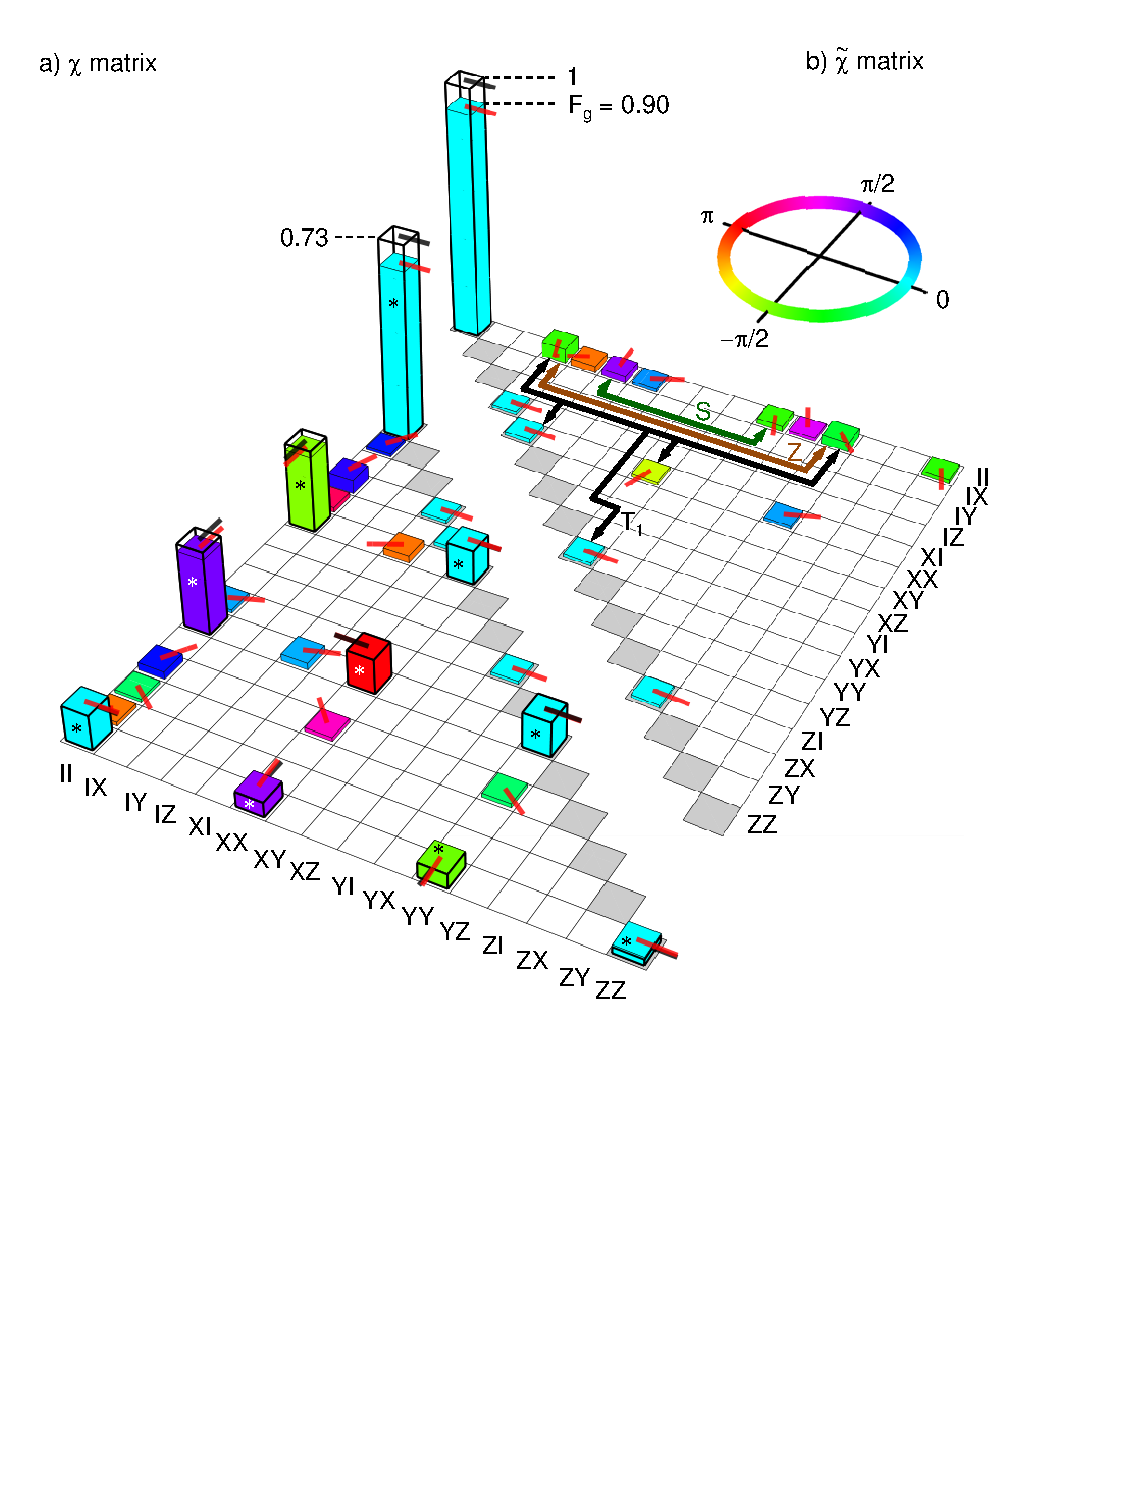
\includegraphics[width=1.\textwidth]{./material/papers/iswap/figures/chi_matrix_and_error_process}
	\label{fig:GateChiMatrixAndErrorProcess}
	\caption{}
\end{figure}

